%%%%%%%%%%%%%%%%%%%%%%%%%%%%%%%%%%%%%%%%%%%%%%%%%%%%%%%%%%%%%%%%%%%%%%%%%%%%
%  第17回 解答［24］〜［30］（旧 prob_p132.png 〜 prob_p136_1.png）
%  ※ このファイルは記録用。実体は physics_ch17.tex に流し込み済み。
%%%%%%%%%%%%%%%%%%%%%%%%%%%%%%%%%%%%%%%%%%%%%%%%%%%%%%%%%%%%%%%%%%%%%%%%%%%%

\KaiTitle{第17回　気体の状態変化\MARU{2}}
\setlength{\columnseprule}{0.4pt}
\begin{multicols}{2}
\raggedcolumns

\Rank{A問題}
\MonN{24}{基本事項の確認}\par\nopagebreak
\begin{sisin}
比熱比の定義式$\gamma=\dfrac{C_P}{C_V}$とマイヤーの関係式$C_P=C_V+R$を利用する．比熱比の分母・分子がどちらにくるかは，\underline{比熱比は}\hskip0pt\underline{必ず$1$}\hskip0pt\underline{より大}\hskip0pt\underline{きい}と覚えておけば間違いがない．
\end{sisin}
\KaiHead
マイヤーの関係式$C_P=C_V+R$を用いると，
\[\gamma=\frac{C_P}{C_V}=1+\frac{R}{C_V}\]
であるから，
\[\text{単原子分子理想気体：}\gamma=1+\frac{R}{\frac{3}{2}R}=\frac{5}{3}\]
\[\text{二原子分子理想気体：}\gamma=1+\frac{R}{\frac{5}{2}R}=\frac{7}{5}\Ans\]

\Rank{B問題}
\MonN{25}{状態変化に伴う各物理量の変化}\par\nopagebreak
\begin{sisin}
各状態変化で，熱量，仕事，内部エネルギーのどれが$0$になるのか（もしくは特殊な値・式となるのか）を覚えておき，残りの量については，$-W=\displaystyle\int_{V_{\mathrm{initial}}}^{V_{\mathrm{final}}}P(V)dV$, $\Delta U=nC_V\Delta T$, $\Delta U=Q+W$の各式から正負を判定する．

状態変化前後の状態方程式の両辺を差し引くと，
\[\begin{array}{r@{\;}l}
       & P_1V_1=nRT_1\\
 -)\;\;& P_0V_0=nRT_0\\ \hline
       & P_1V_1-P_0V_0=nR(T_1-T_0)
\end{array}\]
となる．ここで$PV$の項の変化$P_1V_1-P_0V_0$を$\Delta(PV)$と書くと，
\[\Delta(PV)=nR\cdot\Delta T\]
がすべての状態変化に対して成立する．温度変化についてはこれを利用して考えると便利である．
\end{sisin}
\KaiHead
状態変化前を$(P_0,V_0,T_0)$，変化後を$(P_1,V_1,T_1)$とする．$W$は外部が気体に対してした仕事であるから，気体が外部に対してした仕事は$(-W)$で表され，$-W=\displaystyle\int_{V_{\mathrm{initial}}}^{V_{\mathrm{final}}}P(V)dV$が成り立つ．内部エネルギーは絶対温度にのみ依存し$\Delta U=nC_V\Delta T$と表せる．また，熱力学の第一法則より$\Delta U=Q+W$，変化前後の状態方程式を辺々引いて，$P_1V_1-P_0V_0=nR(T_1-T_0)$が成り立つ．体積変化$\Delta V$を$\Delta V=V_1-V_0$とする．
\begin{komon}
\ko{1} 定圧であるから，$-W=P_0\cdot\Delta V$と表せる．\par
       \hspace*{1zw}圧縮しているので$\Delta V<0$であるから$W>0$，また$P_0\cdot\Delta V<0$であるから温度変化は$\Delta T<0$である．よって$\Delta U<0$となり，$Q=\Delta U+(-W)<0$である．
       \[\text{\MARU{1}負，\MARU{2}正，\MARU{3}負，\MARU{4}下降する}\Ans\]
\ko{2} 定積であるから$\Delta V=0$であり，$W=0$である．\par
       \hspace*{1zw}減圧していくので，$P_1V_0-P_0V_0<0$であるから温度変化は$\Delta T<0$である．よって$\Delta U<0$となり，$Q=\Delta U+(-W)<0$である．以上より，
       \[\text{\MARU{1}負，\MARU{2}$0$，\MARU{3}負，\MARU{4}下降する}\Ans\]
\ko{3} 定温であるから温度が一定であり，$\Delta U=0$である．\par
       \hspace*{1zw}加圧しているので$P_1>P_0$であり，状態方程式$P_1V_1=nRT_0$および$P_0V_0=nRT_0$より$V_1<V_0$, すなわち体積は減少している．よって$W>0$であり，$Q=\Delta U+(-W)<0$である．以上より，
       \[\text{\MARU{1}負，\MARU{2}正，\MARU{3}$0$，\MARU{4}一定である}\Ans\]
       \begin{chuu}
       気体が外部にした仕事$(-W)$の正負は$P-V$図から考えれば明らかである．定温曲線は次図のように双曲線となるのだから，加圧すれば体積は減少する．よって，$-W<0$となるのはこの図より明らか．
       % 誤植訂正（2026-09-02）：原本は「よって，W<0 となるのは…」．
       %   直前で「気体が外部にした仕事 (-W) の正負は」と述べており，加圧＝圧縮
       %   では (-W)<0（したがって W>0）．本解の(3)も「よって W>0 であり」と
       %   しているので，(-W)<0 に改めた．
       \begin{center}
       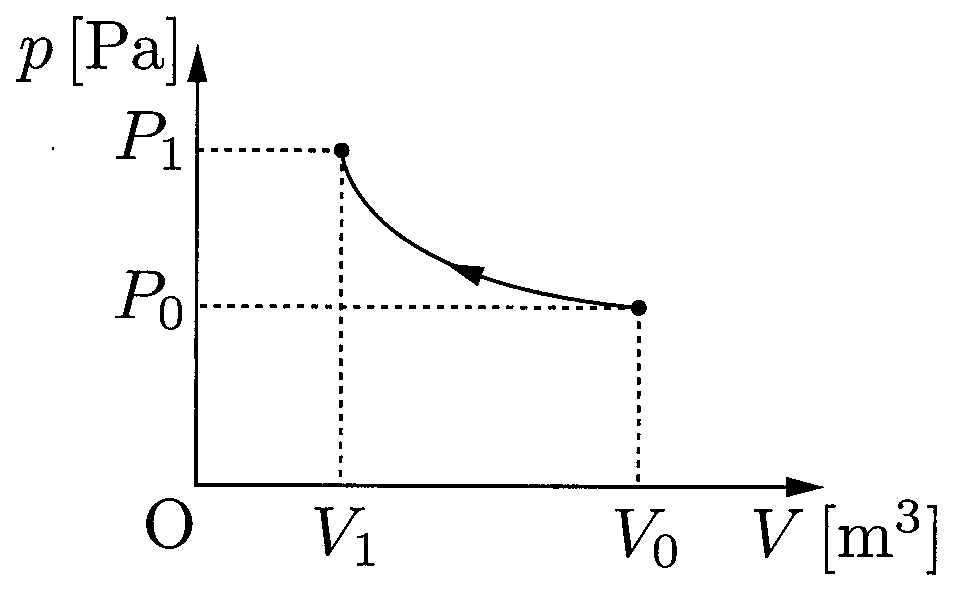
\includegraphics[keepaspectratio,width=54mm]{fig/ch17_a25_pv.png}
       \end{center}
       \end{chuu}
\ko{4} 断熱変化であるから，$Q=0$である．\par
       \hspace*{1zw}圧縮しているので$\Delta V<0$であるから$W>0$，また$\Delta U=Q+W$より$\Delta U>0$であるから温度変化は$\Delta T>0$である．以上より，
       \[\text{\MARU{1}$0$，\MARU{2}正，\MARU{3}正，\MARU{4}上昇する}\Ans\]
       \begin{chuu}
       (1)〜(4)の各状態変化ごとに本質的に覚えておくべきことは最初の一行のみである．あとは指針で述べた関係式から他の物理量の変化が分かる．
       \end{chuu}
\end{komon}

\MonN{26}{定温変化}\par\nopagebreak
\begin{sisin}
本問のように，変化途中で気体の圧力が変化する場合には$w=P\cdot\Delta V$としてはいけない．体積が$V\U{m^3}$のときの圧力$P(V)\U{Pa}$を求め，これを積分することで求める．
\end{sisin}
\KaiHead
\begin{komon}
\ko{1} 最初の状態について状態方程式を立てると，
       \[p_0\cdot Sl_0=nRT_0\]
       であるから，
       \[p_0=\frac{nRT_0}{Sl_0}\U{Pa}\Ans\]
\ko{2} 終状態における状態方程式は，
       \[p_1\cdot Sl_1=nRT_0\]
       であるから，
       \[p_1=\frac{nRT_0}{Sl_1}\U{Pa}\Ans\]
\ko{3} 気体の体積が$V\U{m^3}$のときの気体の圧力を$p(V)\U{Pa}$とし，このときの気体の状態方程式を立てると，
       \[p(V)\cdot V=nRT_0\]
       これより，
       \[p(V)=\frac{nRT_0}{V}\]
       よって，体積が$V=Sl_0\rightarrow Sl_1\U{m^3}$に変化するまでに気体が外部にした仕事$w$は，$nRT_0$が定数であることに注意して
       \[\begin{aligned}
         w&=\int_{Sl_0}^{Sl_1}p(V)dV=\int_{Sl_0}^{Sl_1}\frac{nRT_0}{V}dV\\
          &=nRT_0\int_{Sl_0}^{Sl_1}\frac{1}{V}dV\\
          &=nRT_0\Bigl[\log_e|V|\Bigr]_{Sl_0}^{Sl_1}\\
          &=nRT_0\log_e\frac{l_1}{l_0}\U{J}\Ans
       \end{aligned}\]
\ko{4} この状態変化にて気体の温度は$T_0$一定であるから，気体の内部エネルギー変化$\Delta U\U{J}$は
       \[\Delta U=nC_V\Delta T=0\]
       である．熱力学第一法則より$Q$, $\Delta U$, $w$の間には，
       \[\Delta U=Q+(-w)\]
       の関係が成り立つ．以上より気体に加えた熱量は
       \[Q=nRT_0\log_e\frac{l_1}{l_0}\U{J}\Ans\]
\end{komon}

\MonN{27}{断熱変化}\par\nopagebreak
\begin{sisin}
ピストンはゆっくりと移動するので，この状態変化は準静的過程である．理想気体の均一系準静的断熱変化では，ポアソンの式
\[PV^\gamma=（一定）,\;TV^{\gamma-1}=（一定）\]
が成立する．どちらの式を利用した方がよいかは問題文に与えられている文字で考えよ．本問では$p$, $T$の両方が問われているのでどちらを利用してもよい．前者の$pV^\gamma=（一定）$で考えた場合を示す．

断熱曲線の勾配は等温曲線よりも急になる．

\underline{断熱変化の}\hskip0pt\underline{場合に限}\hskip0pt\underline{り，$w$を}\hskip0pt\underline{熱力学第}\hskip0pt\underline{一法則か}\hskip0pt\underline{ら求める}\hskip0pt\underline{ことがで}\hskip0pt\underline{きる}．断熱変化の場合は$Q=0$であるから，$\Delta U$から$w$を求めることができるのである．もちろん$w=\displaystyle\int_{V_{\mathrm{initial}}}^{V_{\mathrm{final}}}P(V)dV$から求めることも可能である．
\end{sisin}
\KaiHead
気体の比熱比$\gamma$は，マイヤーの関係式を用いて，
\[\gamma=\frac{C_P}{C_V}=\frac{C_V+R}{C_V}=1+\frac{R}{C_V}\]
で与えられる．
\begin{komon}
\ko{1} 初めの状態について状態方程式を立てると，
       \[p_0Sl_0=nRT_0\]
       これを解いて，
       \[p_0=\frac{nRT_0}{Sl_0}\U{Pa}\Ans\]
\ko{2} 気体は外界と熱のやり取りをしておらず，断熱変化であるので，初状態と終状態に対してポアソンの式より，
       \[p_0(Sl_0)^\gamma=p_1(Sl_1)^\gamma\]
       が成り立つ．これを解いて，
       \[p_1=\frac{nRT_0}{Sl_0}\left(\frac{l_0}{l_1}\right)^{1+\frac{R}{C_V}}\U{Pa}\Ans\]
       また，終状態の状態方程式は，
       \[p_1Sl_1=nRT_1\]
       であるから，これを解いて
       \[T_1=T_0\left(\frac{l_0}{l_1}\right)^{\frac{R}{C_V}}\U{K}\Ans\]
       \begin{bekkai}
       もう一つのポアソンの式$TV^{\gamma-1}=$一定を利用してもよい．この場合は，
       \[T_0(Sl_0)^{\gamma-1}=T_1(Sl_1)^{\gamma-1}\]
       より，$T_1=T_0\left(\dfrac{l_0}{l_1}\right)^{\frac{R}{C_V}}\U{K}$を導くことができる．また，この$T_1$を元に終状態の状態方程式$p_1Sl_1=nRT_1$を立てて圧力$p_1$を求めることが可能である．

       ポアソンの式は多少面倒な式であるから，まず$pV^\gamma=$一定もしくは$TV^{\gamma-1}=$一定を用いて変化後の$p$, $T$のいずれか一方を求め，もう片方については状態方程式から求めればよい．両方をポアソンの式から求めるのは面倒なだけである．
       \end{bekkai}
\ko{3} 気体の体積が$V\U{m^3}$のときの気体の圧力を$p(V)\U{Pa}$とし，初状態とこの状態との間にポアソンの式より，
       \[p(V)V^\gamma=p_0(Sl_0)^\gamma\quad(=\text{一定})\]
       が成り立つ．よって，
       \[p(V)=p_0(Sl_0)^\gamma\frac{1}{V^\gamma}\]
       である．ここで$\gamma>1$に注意すると，これは右下がりの曲線を表すので，状態変化の$p-V$図は次図の通り．
       \begin{center}
       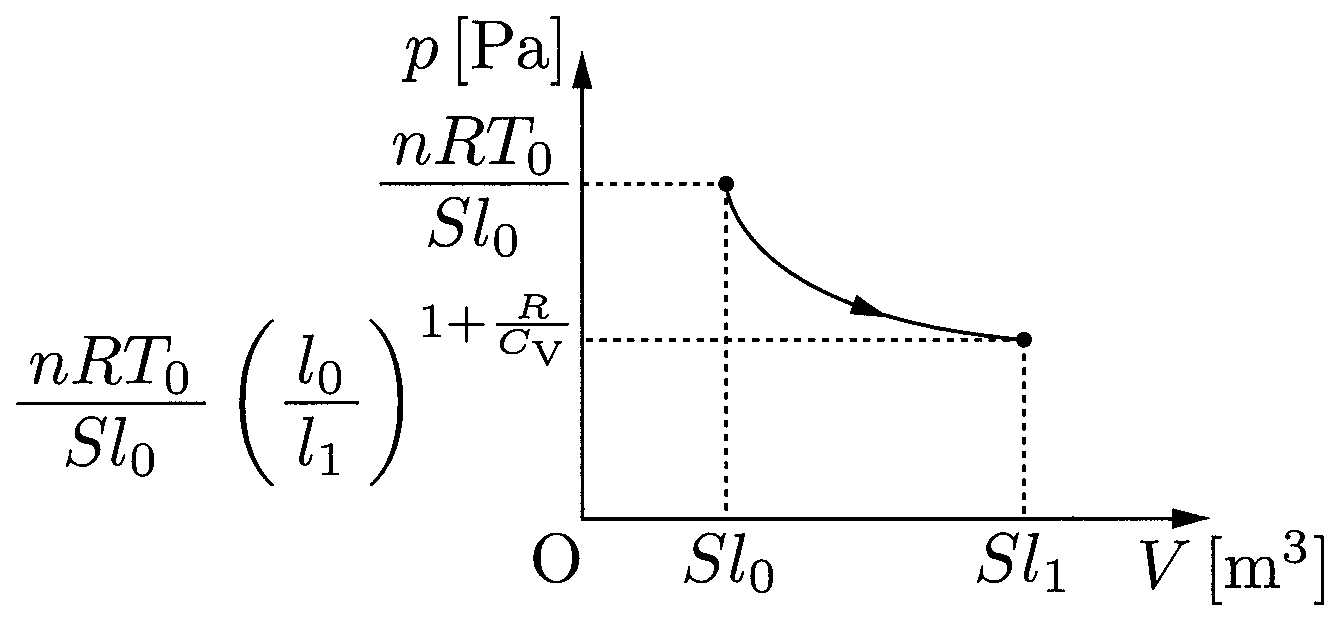
\includegraphics[keepaspectratio,width=64mm]{fig/ch17_a27_pv.png}
       \end{center}
       \hspace*{\fill}\Ans
\ko{4} この変化は断熱変化であるから，外部が気体に与える熱量$Q$は，
       \[Q=0\]
       また，この状態変化の内部エネルギーの増加量$\Delta U$は，
       \[\begin{aligned}
         \Delta U&=nC_V(T_1-T_0)\\
                 &=nC_VT_0\left\{\left(\frac{l_0}{l_1}\right)^{\frac{R}{C_V}}-1\right\}\U{J}
       \end{aligned}\]
       気体が外界に対してした仕事$w$は，熱力学第一法則を用いると，
       \[\Delta U=Q+(-w)\]
       の関係があるので，
       \[\begin{aligned}
         w&=-\Delta U\\
          &=nC_VT_0\left\{1-\left(\frac{l_0}{l_1}\right)^{\frac{R}{C_V}}\right\}\U{J}\Ans
       \end{aligned}\]
       \begin{bekkai}
       指針でも述べたように，まともに
       \[w=\int_{V_{\mathrm{initial}}}^{V_{\mathrm{final}}}P(V)dV\]
       を計算しても同一の答えが求められる．気体の体積が$V\U{m^3}$のときの気体の圧力$p(V)\U{Pa}$は，
       \[p(V)=p_0(Sl_0)^\gamma\frac{1}{V^\gamma}\]
       であるから，
       \[\begin{aligned}
         w&=\int_{Sl_0}^{Sl_1}p(V)dV\\
          &=p_0(Sl_0)^\gamma\int_{Sl_0}^{Sl_1}\frac{1}{V^\gamma}dV\\
          &=p_0(Sl_0)^\gamma\left[\frac{1}{-\gamma+1}V^{-\gamma+1}\right]_{Sl_0}^{Sl_1}\\
          &=p_0(Sl_0)^\gamma\left[-\frac{C_V}{R}\cdot\frac{1}{V^{\gamma-1}}\right]_{Sl_0}^{Sl_1}\\
          &=-\frac{C_V}{R}p_0(Sl_0)^{\gamma-1}(Sl_0)\\
          &\qquad\times\left\{\frac{1}{(Sl_1)^{\gamma-1}}-\frac{1}{(Sl_0)^{\gamma-1}}\right\}\\
          &=-\frac{C_V}{R}p_0(Sl_0)\left\{\left(\frac{l_0}{l_1}\right)^{\gamma-1}-1\right\}\\
          &=\frac{C_V}{R}\frac{nRT_0}{Sl_0}Sl_0\left\{1-\left(\frac{l_0}{l_1}\right)^{\frac{R}{C_V}}\right\}\\
          &=nC_VT_0\left\{1-\left(\frac{l_0}{l_1}\right)^{\frac{R}{C_V}}\right\}\U{J}
       \end{aligned}\]
       となり，全く同じ答えが導ける．しかし，この計算はなかなかに厄介である．断熱変化に限っては熱力学第一法則から$w$を求めることを覚えておくとよい．
       \end{bekkai}
\end{komon}

\MonN{28}{断熱自由膨張}\par\nopagebreak
\begin{sisin}
本問のような断熱自由膨張では，\underline{容器$\mathrm{A+B}$}\hskip0pt\underline{全体を一}\hskip0pt\underline{つの系と}\hskip0pt\underline{みなして}\hskip0pt\underline{熱力学第}\hskip0pt\underline{一法則を}\hskip0pt\underline{立てる}のがポイント．$\mathrm{A+B}$の全体積は$V_\mathrm{A}+V_\mathrm{B}\U{m^3}$のまま不変であるから，$\mathrm{A+B}$は容器外と仕事のやり取りをしない．また，断熱容器を使っているから熱のやり取りもない．以上に着目して熱力学第一法則を立てる．
\end{sisin}
\KaiHead
変化後の$\mathrm{A}$, $\mathrm{B}$内の気体の圧力を$p\U{Pa}$, 温度を$T\U{K}$とする．この変化において，$\mathrm{A+B}$を一つの系とみなすと，これは体積が不変であるから外界と仕事のやり取りをせず，また断熱容器を利用しているので外界と熱のやり取りもしない．よって，内部エネルギーの変化量を$\Delta U$とすると，熱力学第一法則より，
\[\Delta U=0+0\]
と立式できる．$\Delta U$は絶対温度に比例し，
\[\Delta U=nC_V\Delta T=0\]
と表せるので，これより$\Delta T=0$, すなわち気体の温度は変化しない．
\[T=T_0\U{K}\Ans\]
また状態変化前の$\mathrm{A}$内の気体のモル数を$n$とすると，状態方程式は，
\[p_0V_\mathrm{A}=nRT_0\]
また状態変化後は$\mathrm{A+B}$に一様に気体が広がっているので$\mathrm{A+B}$全体に対して状態方程式を立てることができ，
\[p(V_\mathrm{A}+V_\mathrm{B})=nRT_0\]
となる．以上2式を組み合わせて，
\[p=\frac{V_\mathrm{A}}{V_\mathrm{A}+V_\mathrm{B}}p_0\U{Pa}\Ans\]

\MonN{29}{断熱膨張・断熱自由膨張}\par\nopagebreak
\begin{sisin}
(1)も(2)もいずれも断熱変化であり，最終的には全体積$2V_0\U{m^3}$の空間に気体が広がることになるが，(1)の方法と(2)の方法は全く異なる．(1)は前問と全く同じで，真空中への拡散である．一方，(2)は，バルブを全開にしてからゆっくりと引いているのだから，バルブはないのと同じことである．よって，これは準静的な断熱膨張で，ポアソンの式を利用して考えればよい．
\end{sisin}
\KaiHead
気体のモル数を$n\U{mol}$とすると，最初の状態の状態方程式は
\[p_0V_0=nRT_0\]
である．
\begin{komon}
\ko{1} この方法では，次図のようにいったん右側に体積$V_0\U{m^3}$の真空を作り，左側から右側へ気体を拡散させていくので断熱自由膨張だとみなせる．
       \begin{center}
       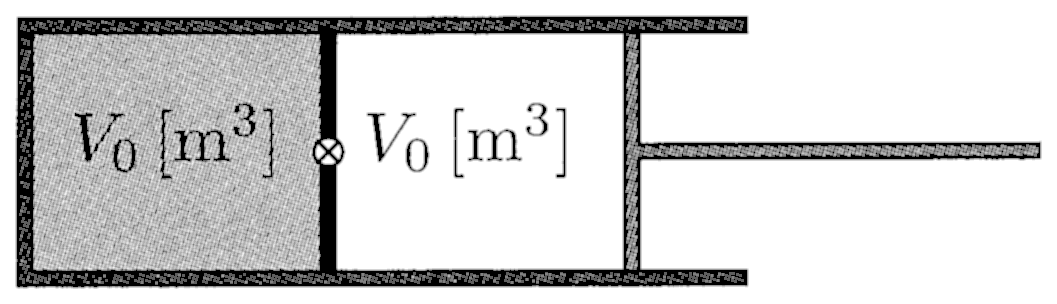
\includegraphics[keepaspectratio,width=62mm]{fig/ch17_a29_1.png}
       \end{center}
       よって，左側の空間と右側の空間を一つの系だとみなすと，この系は外界との仕事のやり取り，熱のやり取りがない．内部エネルギーの変化量を$\Delta U\U{J}$とすると，熱力学第一法則より$\Delta U=0+0$となる．内部エネルギーは絶対温度に比例するので，全体に拡がる前後で温度変化はなく，変化後の気体の温度を$T_1\U{K}$とおくと，
       \[T_1=T_0\U{K}\Ans\]
       また，このときの気体の圧力を$p_1\U{Pa}$とする．最終的には容器全体に気体が一様に拡がっているので，全体に対して状態方程式を立てることができ，
       \[p_1\cdot 2V_0=nRT_0\]
       \begin{center}
       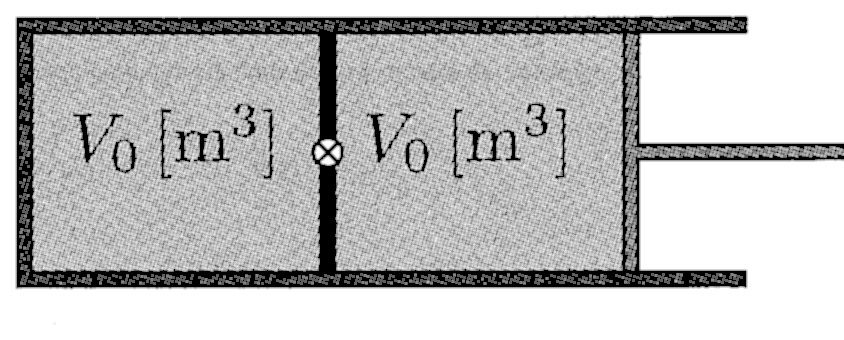
\includegraphics[keepaspectratio,width=54mm]{fig/ch17_a29_2.png}
       \end{center}
       これと最初の状態方程式とを組み合わせて解くと，
       \[p_1=\frac{1}{2}p_0\U{Pa}\Ans\]
\ko{2} バルブを全開にしてから取っ手をゆっくりと引く場合，バルブを通して気体は右側へと十分に拡散することができるので，例えば右側の体積が$V\U{m^3}$となったときには，気体は次の図のように左側と右側とにムラなく広がっている．
       \begin{center}
       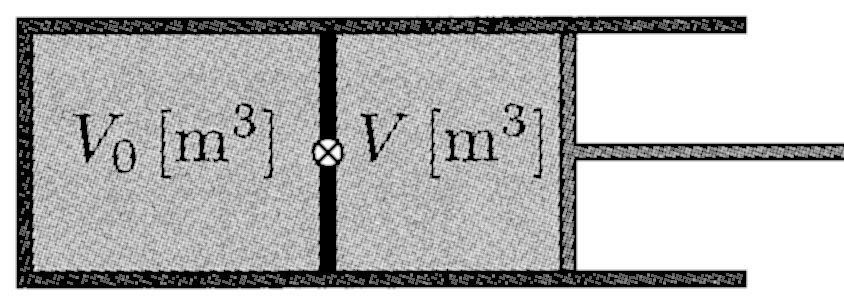
\includegraphics[keepaspectratio,width=54mm]{fig/ch17_a29_3.png}
       \end{center}
       すなわち，この状態変化ではバルブは存在しないのと全く同様にみなせるので，この状態変化は次図と全く同じものとみなせる．
       \begin{center}
       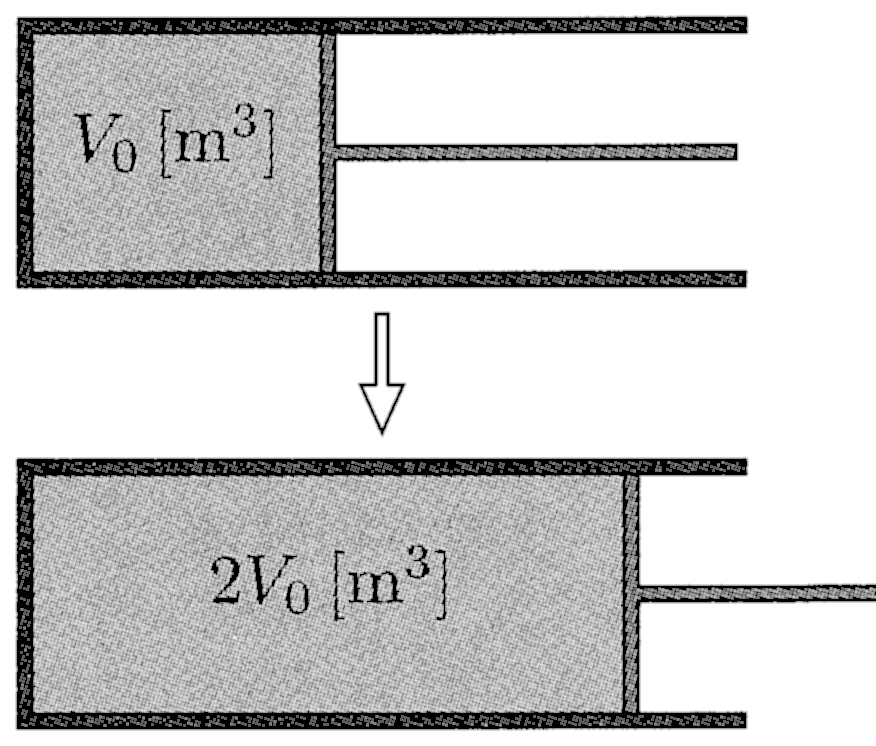
\includegraphics[keepaspectratio,width=52mm]{fig/ch17_a29_4.png}
       \end{center}
       よって，この断熱変化に対してはポアソンの式を適用することができる．この気体の比熱比$\gamma$は
       \[\gamma=\frac{C_P}{C_V}=\frac{C_V+R}{C_V}=1+\frac{R}{C_V}\]
       で与えられるので，終状態の圧力を$p_2\U{Pa}$とすると，ポアソンの式より，
       \[p_0V_0^\gamma=p_2(2V_0)^\gamma\]
       が成立する．これを解いて，
       \[p_2=\frac{1}{2^\gamma}p_0=\frac{1}{2^{1+R/C_V}}p_0\U{Pa}\Ans\]
       また，終状態での温度を$T_2\U{K}$とおくと，状態方程式を立てると，
       \[p_2\cdot 2V_0=nRT_2\]
       よって，
       \[T_2=\frac{1}{2^{R/C_V}}T_0\U{K}\Ans\]
       \begin{bsHosoku}{参考}
       二つの変化それぞれの正しい解法は上述した通りだが，ではなぜ(1)の場合にポアソンの式が利用できないのか？

       それは，(1)の状態変化では，変化途中（すなわち左から右へと気体が拡散している途中）において，気体全体を一つの均一系とみなすことができないからである．

       次の図にあるように，気体が左から右へ拡散していく途中では左の気体の方が気体の密度，圧力が高い．そのため，左，右のそれぞれについて状態方程式を立てることはできるが，左＋右をひとくくりにして状態方程式を立てることができない（圧力が共通ではないから）．
       \begin{center}
       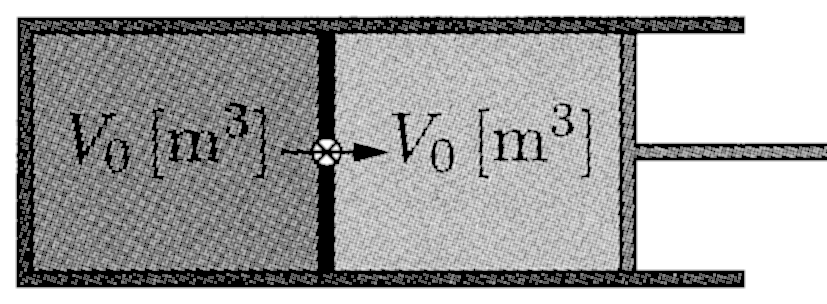
\includegraphics[keepaspectratio,width=54mm]{fig/ch17_a29_ref.png}
       \end{center}
       ポアソンの式の導出では気体全体に対しての状態方程式を利用しているので，(1)のような断熱自由膨張に対してはポアソンの式を利用することができないのである．
       \end{bsHosoku}
\end{komon}

\Rank{C問題}
\MonN{30}{気体の一般的な状態変化}\par\nopagebreak
\begin{sisin}
本問はバネがあるため，気体の状態変化は定積，定圧，定温，断熱のいずれにも当てはまらない．このような場合には，全ての状態変化に対して成立する次の基本的な流れに従って考えよ．
\begin{list}{}{\setlength{\leftmargin}{1.6zw}\setlength{\itemsep}{0.3mm}\setlength{\topsep}{0.6mm}\setlength{\parsep}{0pt}}
\item[\MARU{1}] $w=\displaystyle\int_{V_{\mathrm{start}}}^{V_{\mathrm{end}}}P(V)dV$の計算
\item[\MARU{2}] $\Delta U=nC_V\Delta T$の計算
\item[\MARU{3}] 熱力学第一法則$\Delta U=Q+(-w)$の立式
\end{list}
\end{sisin}
\KaiHead
問題の図にある，バネが距離$x\U{m}$だけ縮んだ途中状態における気体の圧力を$P(x)$とすると，ピストンに対して作用する力のつり合いより，
\[P(x)S=P_0S+kx\]
これより，
\[P(x)=P_0+\frac{kx}{S}\U{Pa}\]
また，このときの体積は
\[V(x)=S(l_0+x)\U{m^3}\]
封入されている気体のモル数を$n\U{mol}$とすると，最初の状態の状態方程式は
\[P_0\cdot Sl_0=nRT_0\]
である．
\begin{komon}
\ko{1} 終状態，すなわち$x=a\U{m}$のときは，
       \[P_1=P(a)=P_0+\frac{ka}{S}\U{Pa}\Ans\]
       であり，このときの気体の状態方程式は
       \[P_1\cdot S(l_0+a)=nRT_1\]
       これと最初の状態の状態方程式を組み合わせて解くと，
       \[T_1=\left(1+\frac{ka}{P_0S}\right)\left(1+\frac{a}{l_0}\right)T_0\U{K}\Ans\]
\ko{2} この状態変化で気体がする仕事は，積分を用いて
       \[w=\int_{Sl_0}^{S(l_0+a)}P(V)dV\]
       で求められる．この式の積分変数を$V$から$x$に変えると，
       \[\frac{dV}{dx}=S\;\Leftrightarrow\;dV=Sdx\]
       \[V=S(l_0+a)\;\Leftrightarrow\;x=a\]
       \[V=Sl_0\;\Leftrightarrow\;x=0\]
       であるから，
       \[\begin{aligned}
         w&=\int_0^a\left(P_0+\frac{kx}{S}\right)Sdx\\
          &=\int_0^a(P_0S+kx)dx\\
          &=P_0Sa+\frac{1}{2}ka^2\U{J}\Ans
       \end{aligned}\]
       \begin{chuu}
       圧力$P$を体積$V$で表してもよい．
       \[P(x)=P_0+\frac{kx}{S}\U{Pa}\]
       \[V(x)=S(l_0+x)\U{m^3}\]
       の2式から$x$を消すと，
       \[P(V)=P_0+\frac{k}{S}\left(\frac{V}{S}-l_0\right)\U{Pa}\]
       が得られる．これをもとに$p-V$図を描き，その面積から仕事を求めることができる．
       \end{chuu}
\ko{3} この状態変化での内部エネルギーの増加は
       \[\Delta U=nC_V(T_1-T_0)\]
       であり，熱力学第一法則$\Delta U=Q+(-w)$を利用すると，
       \[\begin{aligned}
         Q&=nC_VT_0\left(\frac{ka}{P_0S}+\frac{a}{l_0}+\frac{ka^2}{P_0Sl_0}\right)\\
          &\qquad\qquad\qquad+P_0Sa+\frac{1}{2}ka^2\U{J}\\
          &=\frac{C_V}{R}kal_0+\frac{2C_V+R}{2R}ka^2\\
          &\qquad\qquad\qquad+\frac{C_V+R}{R}P_0Sa\U{J}\Ans
       \end{aligned}\]
\end{komon}

\end{multicols}
